% !TEX encoding = UTF-8 Unicode
% !TEX program = pdflatex
\documentclass{article}
	\usepackage{tkz-euclide}
\begin{document}
	$$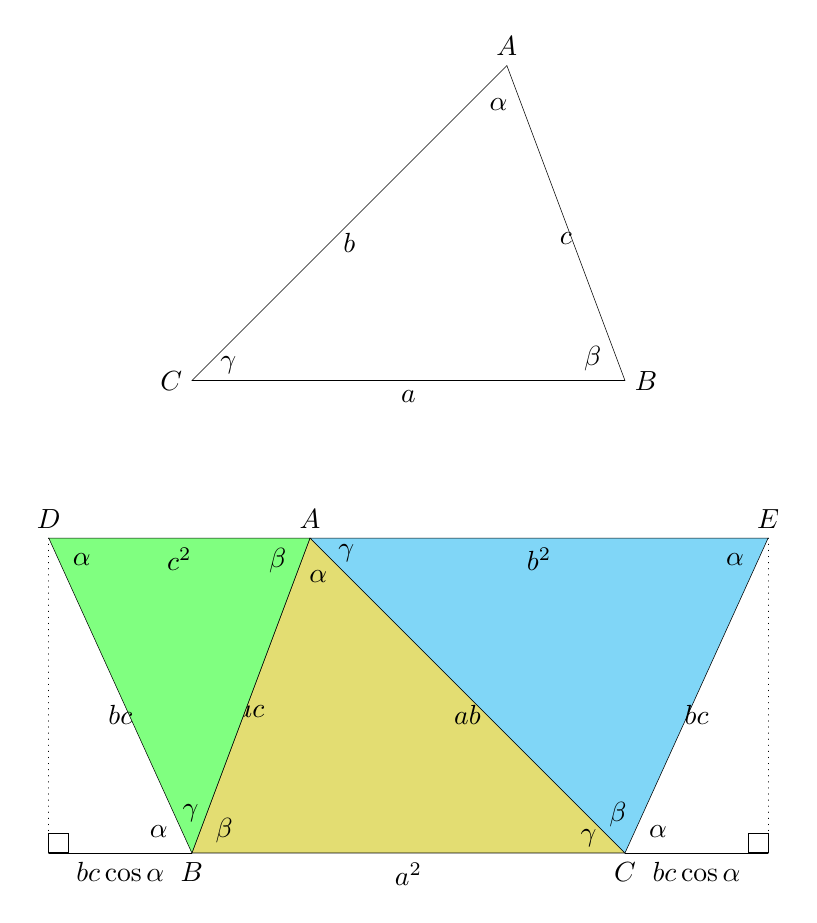
\begin{tikzpicture}
		\def\ya{4}
		\def\xb{1.5}
		\def\xc{-4}
		% the prototype triangle
		\tkzDefPoint(0,\ya){A} \tkzLabelPoint[above](A){$A$}
		\tkzDefPoint(\xb,0){B} \tkzLabelPoint[right](B){$B$}
		\tkzDefPoint(\xc,0){C} \tkzLabelPoint[left](C){$C$}
		\tkzDrawSegment(B,C) \tkzLabelSegments(B,C){$a$}
		\tkzDrawSegment(C,A) \tkzLabelSegments(C,A){$b$}
		\tkzDrawSegment(A,B) \tkzLabelSegments(A,B){$c$}
		\tkzLabelAngle[pos=.5](C,A,B){$\alpha$}
		\tkzLabelAngle[pos=.5](A,B,C){$\beta$}
		\tkzLabelAngle[pos=.5](B,C,A){$\gamma$}
		\tkzFindAngle(C,B,A) \tkzGetAngle{bet}
		\tkzFindAngle(B,C,A) \tkzGetAngle{gam}
		\tikzset{shift={(\xb+\xc, -2-\ya)}}
		% the copy in the middle
		\tkzDefPoint( 0,\ya){A} \tkzLabelPoint[above](A){$A$}
		\tkzDefPoint(-\xb,0){B} \tkzLabelPoint[below](B){$B$}
		\tkzDefPoint(-\xc,0){C} \tkzLabelPoint[below](C){$C$}
		\tkzFillPolygon[color=yellow!50!lightgray](A,B,C) \tkzDrawPolygon(A,B,C)
		\tkzLabelAngle[pos=.5](B,A,C){$\alpha$} \tkzLabelSegments(C,B){$a^2$}
		\tkzLabelAngle[pos=.5](C,B,A){$\beta$}  \tkzLabelSegments(C,A){$ab$}
		\tkzLabelAngle[pos=.5](A,C,B){$\gamma$} \tkzLabelSegments(A,B){$ac$}
		% the copy to the left
		\tkzDefPointBy[rotation=center A angle \bet](B) \tkzGetPoint{D1}
		\tkzDefPointBy[rotation=center B angle \gam](A) \tkzGetPoint{D2}
		\tkzInterLL(A,D1)(B,D2) \tkzGetPoint{D} \tkzLabelPoint[above](D){$D$}
		\tkzFillPolygon[color=green!50!white](A,B,D) \tkzDrawPolygon(A,B,D)
		\tkzLabelAngle[pos=.5](B,D,A){$\alpha$}
		\tkzLabelAngle[pos=.5](D,A,B){$\beta$}  \tkzLabelSegments(B,D){$bc$}
		\tkzLabelAngle[pos=.5](A,B,D){$\gamma$} \tkzLabelSegments(D,A){$c^2$}
		% the copy to the right
		\tkzDefPointBy[rotation=center A angle \gam](C) \tkzGetPoint{E1}
		\tkzDefPointBy[rotation=center C angle \bet](A) \tkzGetPoint{E2}
		\tkzInterLL(A,E1)(C,E2) \tkzGetPoint{E} \tkzLabelPoint[above](E){$E$}
		\tkzFillPolygon[color=cyan!50!white](A,C,E) \tkzDrawPolygon(A,C,E)
		\tkzLabelAngle[pos=.5](A,E,C){$\alpha$}
		\tkzLabelAngle[pos=.5](E,C,A){$\beta$}  \tkzLabelSegments(A,E){$b^2$}
		\tkzLabelAngle[pos=.5](C,A,E){$\gamma$} \tkzLabelSegments(E,C){$bc$}
		% feet
		\tkzDefPointBy[projection=onto B--C](D) \tkzGetPoint{D'}
		\tkzDefPointBy[projection=onto B--C](E) \tkzGetPoint{E'}
		\tkzDrawSegment[dotted](D,D') \tkzMarkRightAngle(D,D',B)
		\tkzDrawSegment[dotted](E,E') \tkzMarkRightAngle(E,E',C)
		\tkzLabelAngle[pos=.5](D,B,D'){$\alpha$}
		\tkzLabelAngle[pos=.5](E',C,E){$\alpha$}
		\tkzDrawSegment(B,D') \tkzLabelSegments(B,D'){$bc\cos\alpha$}
		\tkzDrawSegment(C,E') \tkzLabelSegments(E',C){$bc\cos\alpha$}
	\end{tikzpicture}$$

	$$ a^2 = b^2 + c^2 - 2bc\cos\alpha $$
\end{document}